%!TEX root = ../master.tex
\chapter{Evaluation}\label{ch:evaluation}
This chapter will describe the evaluation process of the finished prototype. The chapter is spilt into three subsections: a planning section, actual evaluation description and analysis of evaluation results. 

\section{Further Context}\label{sec:furthercontext}
\todo{additional functionality: draw on image to change the sound} wut?

\section{Planning of evaluation}
This section will describe the thoughts the project group made before the actual evaluation test were made. The section will show a description of the evaluation tasks and questions there were planned to be asked during the test. 

What do we want out of this test? / what are we testing for / 

\begin{itemize}
\item The user can alter the output by applying filters.
\item The user understands the interface  
\item The prototypes usability is over 80 percent of the users satisfaction.
\end{itemize}

Possible Interview questions
\begin{itemize}
\item What did you experience when manipulating with the sliders?
\item Where you confused about the design?
\item was the “text” helpfull to you?
\item Any other thoughts?
\end{itemize}

Assignments for the user to solve during the test 
\begin{itemize}
\item Turn on echo
\item Turn on echo and comb
\item Turn off comb
\item Turn on bandpass 
\end{itemize}


The test set up was planned to be held in a quiet area with one test participant at the time, located at Rendensburgade (The Create building) it was planned to conduct the test on at least 12 people (2 test people pr. group member) 


Technical evaluation 



\section{Evaluation test}
This section will give a description of the set-up, procedure and results of the actual evaluation test of the final device. 

\begin{figure}[!h] 
\centering
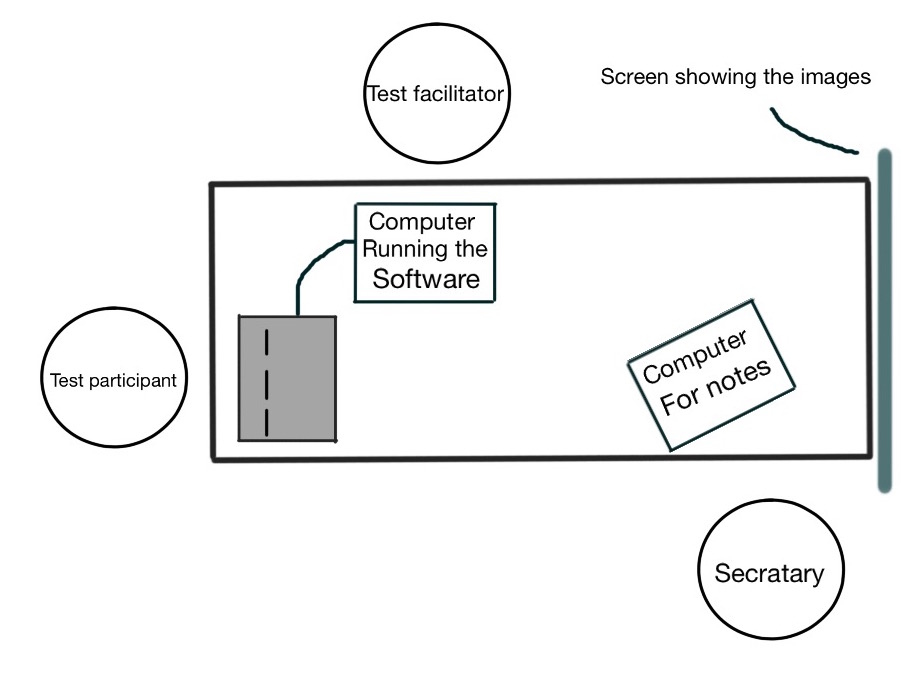
\includegraphics[width=1\textwidth]{testsetup}
\caption{\label{fig:testsetup} Illustration of the test set-up.}
\end{figure}

The final test was conducted on 15 test participants from Aalborg University in their 20's. The participants consisted of 14 students from medialogy and one student from Art \& Technology. \todo{dette kan bruges i diskution, da vi ville have faaet mere variation i resultaterne hvis vi fx. havde testet paa museumsgaester i alle aldre} The test took place in a small closed room located at Rendsburggade 14. The test was conducted by a test facilitator; who interviewed the participants and instructed which tasks to perform while observing the software during the test. During the testing a secretary would take notes of the entire test. Furthermore, the prototype was placed in front of the participants and a laptop was used to display the two pictures the project group decide to use during the test. The facilitator would change the picture on the laptop since it was not automatised and worked independently from the actual software and was only used to display the pictures.   

\begin{figure}[!h] 
\centering
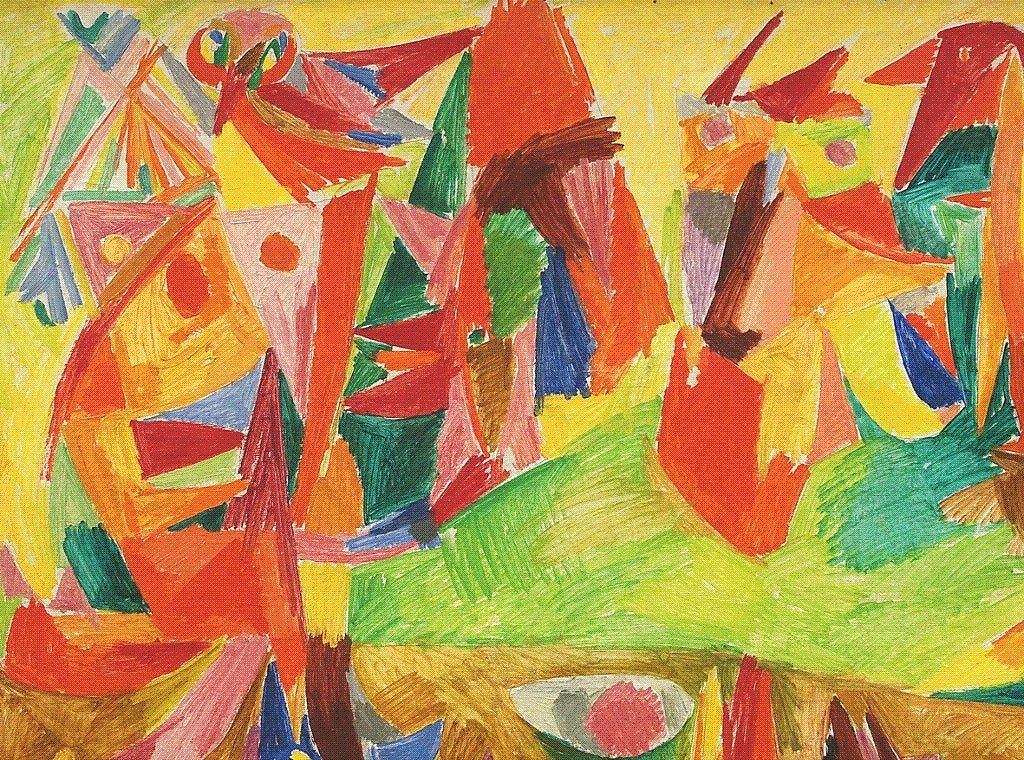
\includegraphics[width=1\textwidth]{asger}
\caption{\label{fig:asger} Asger Jorns "Trolden og Fuglene" 1944.}
\end{figure}

\begin{figure}[!h] 
\centering
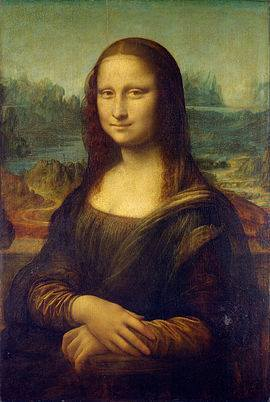
\includegraphics[width=0.5\textwidth]{monalisa}
\caption{\label{fig:monalisa} Leonardo Da Vinci "Mona Lisa" 1503-1517.}
\end{figure}

The test was carried out by welcoming the test participants in the room, one at the time. The participants were places at the end of the table and was asked to sign a consent form. The facilitator then started the test by introducing the overall project and explaining what the participant was expected to do during the test. The facilitator conducted the test by using the script shown below:


\section{Script}
The following text is the actual script, followed during the test.

Hello and thank you for wanting to participate in this test. We are group 30.

Our prototype takes an image and turns it into a sound. During this test we will give you a few different assignments and ask you questions during the test. This is a test of the product, and we prefer you to think out loud during the test.

//Mona Lisa is shown on the screen 
Questions: 


\begin{itemize}
\item What do you think you have to do with this product?
\item What happens when you manipulated with the sliders?
\item Can you hear a difference between “MIN” and “MAX”?
\item Can you hear a difference between the effects?
\item Is the “help text” helpfull to you?
\item Is the help text clear?
\item Any other thoughts?
\end{itemize}



/* Now we will change the images to Asgar Jorn */
\begin{itemize}
\item Do you hear the difference between the two pictures?
\item Why do you think there is a difference between the images?
\item Can you hear a difference between “MIN” and “MAX”?
\item Can you hear a difference between the effects?
\end{itemize}


Any other overall thoughts?


\section{Evaluation results}
This section describes the results found in the final test. The results were found by making a semi-structured interview and getting qualitative feedback by communicating directly with the user, using the script shown above. 

From the testing, 13 of the participants found it difficult to hear the difference between "MIN" and "MAX" when manipulating with the comb filter on both Mona Lisa and Asger Jorns picture. However, when using the Bandpass and High shelf, the user could hear a clear difference between the two filters when changing the values using the sliders. Two of the test participants had no clear comments regarding the difference between any of the filters. These answers was marked as "not clear for use" in case the test facilitator and secretary had misunderstood the participant's answer. 

Nine of the participants did not know the terms of the different filters, but they could distinguish a change in the output when manipulating with the sliders. Therefore, they did not know exactly what to listen for when manipulating with the sliders. Six of the participants from Medialogy knew the terms of the three filters. Even though six of the participants knew the terms of the filters, only two knew exactly what the filters did, and what they had to listen for when manipulating with the sliders. 

The interface was clear for all the participants and they knew how to use it, either by looking at the help text or at the sliders. None of the test participants had any trouble manipulating with the sliders. 

All of the participants could hear a clear difference between the colourful Asger Jorn painting and the darker Mona Lisa painting. They all suspected the difference in the colours for being the reason for the difference in the sound. 

To sum up the overall thoughts on the product, the test participants found the device to be very easy to use, even though most of them did not know what the filters actually did or what the names of the filters meant. 

\todo {One particpant was asking if the later iteration would show the context between the picture and sound to find a balanced and satisfying output}. 